
\documentclass[a4paper,11pt]{article}
\usepackage[a4paper, margin=8em]{geometry}

% usa i pacchetti per la scrittura in italiano
\usepackage[french,italian]{babel}
\usepackage[T1]{fontenc}
\usepackage[utf8]{inputenc}
\frenchspacing 

% usa i pacchetti per la formattazione matematica
\usepackage{amsmath, amssymb, amsthm, amsfonts}

% usa altri pacchetti
\usepackage{gensymb}
\usepackage{hyperref}
\usepackage{standalone}

\usepackage{colortbl}

\usepackage{xstring}
\usepackage{karnaugh-map}

% imposta il titolo
\title{Appunti Calcolatori Elettronici}
\author{Luca Seggiani}
\date{2025}

% imposta lo stile
% usa helvetica
\usepackage[scaled]{helvet}
% usa palatino
\usepackage{palatino}
% usa un font monospazio guardabile
\usepackage{lmodern}

\renewcommand{\rmdefault}{ppl}
\renewcommand{\sfdefault}{phv}
\renewcommand{\ttdefault}{lmtt}

% circuiti
\usepackage{circuitikz}
\usetikzlibrary{babel}

% testo cerchiato
\newcommand*\circled[1]{\tikz[baseline=(char.base)]{
            \node[shape=circle,draw,inner sep=2pt] (char) {#1};}}

% disponi il titolo
\makeatletter
\renewcommand{\maketitle} {
	\begin{center} 
		\begin{minipage}[t]{.8\textwidth}
			\textsf{\huge\bfseries \@title} 
		\end{minipage}%
		\begin{minipage}[t]{.2\textwidth}
			\raggedleft \vspace{-1.65em}
			\textsf{\small \@author} \vfill
			\textsf{\small \@date}
		\end{minipage}
		\par
	\end{center}

	\thispagestyle{empty}
	\pagestyle{fancy}
}
\makeatother

% disponi teoremi
\usepackage{tcolorbox}
\newtcolorbox[auto counter, number within=section]{theorem}[2][]{%
	colback=blue!10, 
	colframe=blue!40!black, 
	sharp corners=northwest,
	fonttitle=\sffamily\bfseries, 
	title=Teorema~\thetcbcounter: #2, 
	#1
}

% disponi definizioni
\newtcolorbox[auto counter, number within=section]{definition}[2][]{%
	colback=red!10,
	colframe=red!40!black,
	sharp corners=northwest,
	fonttitle=\sffamily\bfseries,
	title=Definizione~\thetcbcounter: #2,
	#1
}

% disponi codice
\usepackage{listings}
\usepackage[table]{xcolor}

\definecolor{codegreen}{rgb}{0,0.6,0}
\definecolor{codegray}{rgb}{0.5,0.5,0.5}
\definecolor{codepurple}{rgb}{0.58,0,0.82}
\definecolor{backcolour}{rgb}{0.95,0.95,0.92}

\lstdefinestyle{codestyle}{
		backgroundcolor=\color{black!5}, 
		commentstyle=\color{codegreen},
		keywordstyle=\bfseries\color{magenta},
		numberstyle=\sffamily\tiny\color{black!60},
		stringstyle=\color{green!50!black},
		basicstyle=\ttfamily\footnotesize,
		breakatwhitespace=false,         
		breaklines=true,                 
		captionpos=b,                    
		keepspaces=true,                 
		numbers=left,                    
		numbersep=5pt,                  
		showspaces=false,                
		showstringspaces=false,
		showtabs=false,                  
		tabsize=2
}

\lstdefinestyle{shellstyle}{
		backgroundcolor=\color{black!5}, 
		basicstyle=\ttfamily\footnotesize\color{black}, 
		commentstyle=\color{black}, 
		keywordstyle=\color{black},
		numberstyle=\color{black!5},
		stringstyle=\color{black}, 
		showspaces=false,
		showstringspaces=false, 
		showtabs=false, 
		tabsize=2, 
		numbers=none, 
		breaklines=true
}


\lstdefinelanguage{assembler}{ 
  keywords={AAA, AAD, AAM, AAS, ADC, ADCB, ADCW, ADCL, ADD, ADDB, ADDW, ADDL, AND, ANDB, ANDW, ANDL,
        ARPL, BOUND, BSF, BSFL, BSFW, BSR, BSRL, BSRW, BSWAP, BT, BTC, BTCB, BTCW, BTCL, BTR, 
        BTRB, BTRW, BTRL, BTS, BTSB, BTSW, BTSL, CALL, CBW, CDQ, CLC, CLD, CLI, CLTS, CMC, CMP,
        CMPB, CMPW, CMPL, CMPS, CMPSB, CMPSD, CMPSW, CMPXCHG, CMPXCHGB, CMPXCHGW, CMPXCHGL,
        CMPXCHG8B, CPUID, CWDE, DAA, DAS, DEC, DECB, DECW, DECL, DIV, DIVB, DIVW, DIVL, ENTER,
        HLT, IDIV, IDIVB, IDIVW, IDIVL, IMUL, IMULB, IMULW, IMULL, IN, INB, INW, INL, INC, INCB,
        INCW, INCL, INS, INSB, INSD, INSW, INT, INT3, INTO, INVD, INVLPG, IRET, IRETD, JA, JAE,
        JB, JBE, JC, JCXZ, JE, JECXZ, JG, JGE, JL, JLE, JMP, JNA, JNAE, JNB, JNBE, JNC, JNE, JNG,
        JNGE, JNL, JNLE, JNO, JNP, JNS, JNZ, JO, JP, JPE, JPO, JS, JZ, LAHF, LAR, LCALL, LDS,
        LEA, LEAVE, LES, LFS, LGDT, LGS, LIDT, LMSW, LOCK, LODSB, LODSD, LODSW, LOOP, LOOPE,
        LOOPNE, LSL, LSS, LTR, MOV, MOVB, MOVW, MOVL, MOVSB, MOVSD, MOVSW, MOVSX, MOVSXB,
        MOVSXW, MOVSXL, MOVZX, MOVZXB, MOVZXW, MOVZXL, MUL, MULB, MULW, MULL, NEG, NEGB, NEGW,
        NEGL, NOP, NOT, NOTB, NOTW, NOTL, OR, ORB, ORW, ORL, OUT, OUTB, OUTW, OUTL, OUTSB, OUTSD,
        OUTSW, POP, POPL, POPW, POPB, POPA, POPAD, POPF, POPFD, PUSH, PUSHL, PUSHW, PUSHB, PUSHA, 
				PUSHAD, PUSHF, PUSHFD, RCL, RCLB, RCLW, MOVSL, MOVSB, MOVSW, STOSL, STOSB, STOSW, LODSB, LODSW,
				LODSL, INSB, INSW, INSL, OUTSB, OUTSL, OUTSW
        RCLL, RCR, RCRB, RCRW, RCRL, RDMSR, RDPMC, RDTSC, REP, REPE, REPNE, RET, ROL, ROLB, ROLW,
        ROLL, ROR, RORB, RORW, RORL, SAHF, SAL, SALB, SALW, SALL, SAR, SARB, SARW, SARL, SBB,
        SBBB, SBBW, SBBL, SCASB, SCASD, SCASW, SETA, SETAE, SETB, SETBE, SETC, SETE, SETG, SETGE,
        SETL, SETLE, SETNA, SETNAE, SETNB, SETNBE, SETNC, SETNE, SETNG, SETNGE, SETNL, SETNLE,
        SETNO, SETNP, SETNS, SETNZ, SETO, SETP, SETPE, SETPO, SETS, SETZ, SGDT, SHL, SHLB, SHLW,
        SHLL, SHLD, SHR, SHRB, SHRW, SHRL, SHRD, SIDT, SLDT, SMSW, STC, STD, STI, STOSB, STOSD,
        STOSW, STR, SUB, SUBB, SUBW, SUBL, TEST, TESTB, TESTW, TESTL, VERR, VERW, WAIT, WBINVD,
        XADD, XADDB, XADDW, XADDL, XCHG, XCHGB, XCHGW, XCHGL, XLAT, XLATB, XOR, XORB, XORW, XORL},
  keywordstyle=\color{blue}\bfseries,
  ndkeywordstyle=\color{darkgray}\bfseries,
  identifierstyle=\color{black},
  sensitive=false,
  comment=[l]{\#},
  morecomment=[s]{/*}{*/},
  commentstyle=\color{purple}\ttfamily,
  stringstyle=\color{red}\ttfamily,
  morestring=[b]',
  morestring=[b]"
}

\lstset{language=assembler, style=codestyle}

% disponi sezioni
\usepackage{titlesec}

\titleformat{\section}
	{\sffamily\Large\bfseries} 
	{\thesection}{1em}{} 
\titleformat{\subsection}
	{\sffamily\large\bfseries}   
	{\thesubsection}{1em}{} 
\titleformat{\subsubsection}
	{\sffamily\normalsize\bfseries} 
	{\thesubsubsection}{1em}{}

% tikz
\usepackage{tikz}

% float
\usepackage{float}

% grafici
\usepackage{pgfplots}
\pgfplotsset{width=10cm,compat=1.9}

% disponi alberi
\usepackage{forest}

\forestset{
	rectstyle/.style={
		for tree={rectangle,draw,font=\large\sffamily}
	},
	roundstyle/.style={
		for tree={circle,draw,font=\large}
	}
}

% disponi algoritmi
\usepackage{algorithm}
\usepackage{algorithmic}
\makeatletter
\renewcommand{\ALG@name}{Algoritmo}
\makeatother

% disponi numeri di pagina
\usepackage{fancyhdr}
\fancyhf{} 
\fancyfoot[L]{\sffamily{\thepage}}

\makeatletter
\fancyhead[L]{\raisebox{1ex}[0pt][0pt]{\sffamily{\@title \ \@date}}} 
\fancyhead[R]{\raisebox{1ex}[0pt][0pt]{\sffamily{\@author}}}
\makeatother

\begin{document}
% sezione (data)
\section{Lezione del 03-03-25}

% stili pagina
\thispagestyle{empty}
\pagestyle{fancy}

% testo
\subsection{Video}
Il supporto principale al video è la \textbf{memoria video}, che lato software si comporta perlopiù come una normale memoria ad accesso casuale.

Questo è quindi il primo esempio di un oggetto che si trova nello spazio di memoria, senza necessariamente \textit{essere} memoria: ciò che vi viene scritto non viene memorizzato, ma visualizzato sullo schermo.

Inoltre, la memoria video supporta un accesso \textit{bidirezionale}: cioè vi si può accedere sia lato CPU che lato \textbf{adattatore video}, cioè la rete che si occupa di gestire tale memoria e visualizzarla sul \textit{display}.
Lo standard VGA usato dal PC IBM prevede che l'adattatore sia configurabile e utilizzabile in due modalità:
\begin{itemize}
	\item \textbf{Modalità testo:} ogni locazione viene associata ad un carattere ASCII da visualizzare sullo schermo, diviso in 80 colonne $\times$ 25 righe (con un carattere di 9 $\times$ 16 pixel, per una risoluzione totale di 720 $\times$ 400 pixel a 70 Hz). È questa la modalità di default in cui si avvia l'adattatore.

		In questo caso il compito dell'adattatore è quello di leggere i 4 KB di memoria, e convertire ogni codice nel carattere principale.
		Questo viene fatto consultando una ROM di caratteri che contiene quello che è effettivamente il carattere (\textit{font}) dell'adattatore.
		Solitamente si può anche redirezionare la lettura in ROM ad una certa regione della RAM, modificando così il font.

		La faccenda è veramente più complicata: si dedicano non 1 ma 2 byte ad ogni carattere, dove il byte più significativo rappresenta informazioni riguardo al \textbf{colore} del carattere:
		\begin{itemize}
			\item I 4 bit meno significativi rappresentano il colore del \textit{foreground};
			\item I 3 bit successivi rappresentano il colore del \textit{background};
				\item Il bit più significativo rappresenta il \textit{blinking}, cioè indica all'adattatore di far \textit{lampeggiare} quel carattere nel tempo.
		\end{itemize}
		Il layout dei flag è quindi:
		\begin{center}
			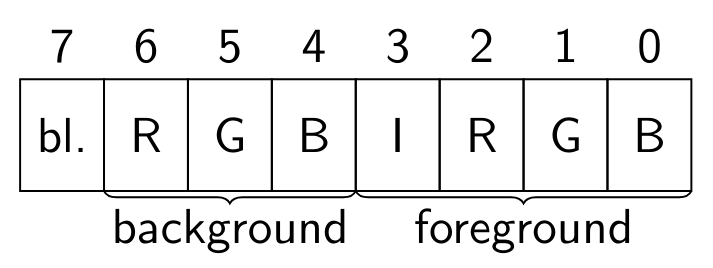
\includegraphics[scale=0.4]{../figures/char_flags.png}
		\end{center}

		Parliamo quindi del \textbf{cursore} comunemente visualizzato sullo schermo nelle interfacce a riga di comando.
		La modalità testo non ha idea della posizione del cursore sullo schermo: attraverso registri si può indicare la posizione del cursore, e modificando la regione di memoria interessata si possono cambiare i caratteri in qualsiasi zona dello schermo.
		Il comportamento del cursore (spostamento, ritorno a capo, ritorno carrello, ecc...) è quindi gestito interamente lato software.
	\item \textbf{Modalità grafica:} programmando i registri dell'adattatore si possono ottenere diverse modalità grafiche, che permettono al progammatore di colorare singoli pixel sul display.
		Le modalità più popolari di questo tipo su schede VGA erano o a 640 $\times$ 400 pixel a 70 Hz (fase di boot grafica), o a 640 $\times$ 480 pixel a 60 Hz non interlacciati (la modalità di default di Microsoft Windows). 
	Nella macchina virtuale usata incapsuliamo tale operazione di conversione in un apposita libreria, e scriviamo pixel con colori su 8 bit (per 256 colori diversi).
	Nei sistemi moderni la memoria video non viene scritta dalla CPU, ma da un \textit{coprocessore grafico} che esegue un suo programma, mentre la CPU può dedicarsi ad altro.	
\end{itemize}

\subsubsection{Indirizzamento dei registri dell'adattatore video}
Vediamo nel dettaglio come si possono indirizzare i registri interni dell'adattatore video.
Questo dispone infatti di una vasta gamma di registri, ma una sola linea di ingresso da un byte per indirizzamento e scrittura.
Le scritture vengono quindi eseguite inserie:
\begin{itemize}
	\item Prima specificando l'\textbf{indirizzo} del registro da aggiornare;
	\item Poi inserendo i \textbf{dati} da scrivere a tale indirizzo.
\end{itemize}

\par\smallskip

Vediamo quindi un programma di esempio che sfrutta l'adattatore grafico in modalita testo a 25 $\times$ 80 caratteri.
Dalla libreria \lstinline|libce| si è importata la variabile \lstinline|video|, che rappresenta l'intero buffer da 4 KB di memoria video (2 byte per cella) a disposizione dall'adattotore.
Le scritture vengono fatte, come avevamo detto, sovrascrivendo dati in tale buffer, mantenendo \textit{lato software} un cursore che ci indica la posizione sullo schermo.

\lstset{style=codestyle, language=c++}
\lstinputlisting{../code/interfaces/video/video.cpp}

\subsection{Timer}
Il timer è realizzato come un interfaccia ad eventi, che riceve in ingresso un clock e aggiorna ciclicamente un registro contatore.
Al raggiungimento di 0 da parte del contatore, si resetta e si invia un certo evento (un impulso).

Nel PC IBM in particolare troviamo 3 contatori:
\begin{itemize}
	\item \textbf{Contatore 0:} è collegata al controllore delle interruzioni;
	\item \textbf{Contatore 1:} era storicamente usato per il refresh della RAM, oggi non viene più usato;
	\item \textbf{Contatore 2:} era collegato all'unico dispositivo audio presente sull'IBM, cioè il beeper speaker.
\end{itemize}

Le porte del timer sono le seguenti:
\begin{table}[h!]
	\center
	\begin{tabular} { c | p{7cm} }
		\lstinline|0x40| & Timer 0 (registro contatore) \\
		\lstinline|0x41| & Timer 1 \hspace{1.2cm} // \\
		\lstinline|0x42| & Timer 2 \hspace{1.2cm} // \\
		\lstinline|0x43| & \textbf{CWR}, \textit{Command Word Register} \\
		\hline
		... & \\
		\hline
		\lstinline|0x61| & \textbf{SPR}, \textit{Speaker Register} \\
	\end{tabular}
\end{table}

Il timer dispone di una vasta gamma di parametri e di solo 2 piedini di indirizzo, quindi 4 locazioni nello spazio di I/O (il controllo speaker si considera a parte), che sono \textbf{CWR}, un registro comune di configurazione delle interfacce, più 4 registri per timer collegati ad ognuna delle 3 porte rimanenti.
L'accesso ai registri di un singolo timer va quindi fatto, cosa interessante del chip, in serie, modificando la stessa porta 1 o 2 volte consecutivamente.

\subsubsection{Sonoro}
Vediamo in particolare il lato sonoro del PC IBM.
Essendo stato questo un calcolatore pensato per l'uso da ufficio, le capabilità audio erano molto limitata: si disponeva di un beeper speeker a frequenza modulabile dal timer (contatore 2).
Inoltre, un particolare registro in memoria era collegato direttamente in AND con l'uscita del contatore 2, permettendo la modulazione on/off del segnale allo speaker.
La modulazione in volume del pc speaker, in particolare, viene fatta attraverso un ulteriore registro detto \textbf{SPR}.

Questo tipo di modulazione permetteva effettivamente di sfruttare, in maniera non prevista dalla IBM, per riprodurre segnali generici.

Mostriamo un esempio di un programma per la riproduzione di un brano musicale monofonico, inteso come una sequenza di note:

\lstinputlisting{../code/interfaces/timer/clean/clean_timer.cpp}

In particolare, il programma si basa sullo scorrimento di un array di strutture \lstinline|song_frame| (definite in \lstinline|song.h|, la cui struttura non ci interessa) ad intervalli regolari.
Questi intervalli vengono ottenuti configurando il timer 0 per oscillare in modalità 2 (oscillazione a onda quadra) con un divisore di 65536, che per un clock a 1.19 MHz fa:
$$
\frac{1.19 \, \mathrm{MHz}}{65536} \approx 17.158 \, \mathrm{Hz}
$$

Lato software, si aspettano 3 di queste oscillazioni, per ottenere una frequenza di $\approx \, 6 \mathrm{Hz}$ (abbastanza vicina a quella delle crome a 120 BPM).

Una volta ottenuto il frame, quindi, si aggiorna il timer 2 di conseguenza, sfruttando il registro SPR per il volume della nota (qui solo on/off) e il suo registro di scrittura per la nota stessa.

\end{document}
